\documentclass[11pt]{beamer}
\usepackage{physics, amsmath, amssymb, mathtools, latexsym, amsfonts, scalefnt}
\usepackage{tikz, lipsum, lmodern, wrapfig, svg, subcaption}
\usepackage[backend=biber, style=alphabetic]{biblatex}
\usepackage[most]{tcolorbox}
\usetheme{EastLansing}
\usecolortheme{beaver}
\usepackage{epigraph}

\title[Bounds on Lyapunov-Schmidt reduction]
      {Estimates on the domain of validity for Lyapunov-Schmidt reduction}

\subtitle{63rd IEEE Conference on Decision and Control, 2024}

\author
[
    \textcolor{yellow}{Pranav~Gupta} \and
    A.~Bizyaeva \and
    R.~Banavar
]
{
    \alert{P.~Gupta \inst{1}}   \and
    A.~Bizyaeva     \inst{2}    \and
    R.~Banavar      \inst{1}
}

\institute[]
{
    \inst{1}
    Indian Institute of Technology Bombay\and
    \inst{2}
    Cornell University
}

\date{December 17, 2024}

\addbibresource{ref.bib}

\begin{document}
\maketitle

\begin{frame}{Contents}
    \tableofcontents
\end{frame}


\begin{frame}{\section{Notations and Definitions}Notations and Definitions}
    \begin{itemize}
        \itemsep2.2mm
        % \item \(\mathbb{R}\equiv\) set of real numbers.
        % \item \(\mathbb{N}\equiv\) set of positive integers.
        \item \(\mathbf{f}\in\mathcal{C}^\nu(\nu\in\mathbb{N})\equiv\nu-\)times continuously differentiable map
        \item \(D_{\mathbf{x}}\mathbf{f}\equiv\) Jacobian matrix \(\begin{bmatrix}\pdv{f_i}{x_j}\end{bmatrix}\) of map \(\mathbf{f}\) with respect to \(\mathbf{x}\).
        \item \(\mathcal{B}(\mathbf{x}_0,r) = \{\mathbf{x}\in\mathbb{R}^n:\norm{\mathbf{x}-\mathbf{x}_0}<r\}\equiv\) open ball of radius \(r>0\) centred at \(\mathbf{x}_0 \in \mathbb{R}^n\) where \(\norm{\cdot}\) is a vector norm on \(\mathbb{R}^n\).
        \item \(\norm{A} := \sup\{\norm{A\mathbf{x}}:\norm{\mathbf{x}}=1\}\equiv\) matrix norm induced by vector norm.
        \item \({\mathcal{N}}(\mathbf{x})\equiv\) an open neighbourhood of \(\mathbf{x}\).
        \item \(\tanh(\mathbf{x}) := \begin{bmatrix} \tanh(x_1) & \dots & \tanh(x_n) \end{bmatrix}^\top\) for \(\mathbf{x} \in \mathbb{R}^n\).
        % \item all mentions of projections and complements are orthogonal in nature.
    \end{itemize}
\end{frame}


\begin{frame}{\section{Introduction}Introduction}
    \begin{columns}
        \hfill
        \begin{column}{0.3\textwidth}
            \begin{figure}[ht!]
                \centering
                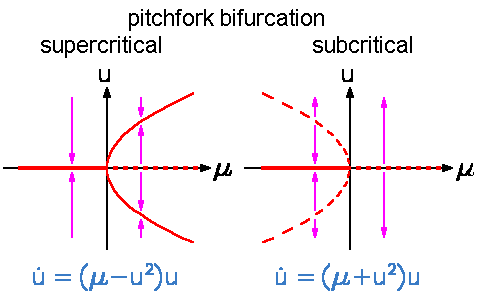
\includegraphics[width=\textwidth]{images/pitchfork.png}
                \caption{pitchfork bifurcation in \(2-\dim\) system occurs along lower \(1-\dim\) manifold; nature and number of equilibria change across \(\mu=0\)}
            \end{figure}
        \end{column}
        \hspace{-5mm}
        \begin{column}{0.75\textwidth}
            \begin{itemize}
                \itemsep1em
                \item \textbf{Bifurcation}: point in a parametrised non-linear dynamical system across which it undergoes \alert{qualitative changes in dynamic behaviour} \cite{guckenheimer2013nonlinear}\footnotemark[1].
                % \item Transition in nature of equilibria, creation of multiple equilibria, onset of oscillation, chaotic dynamics, etc. .
                % \item High dimension state system \(\to\) low dimension bifurcation manifold.
                \item \textbf{Lyapunov-Schmidt reduction}: \alert{dimensionality reduction} technique in non-linear systems analysis, used in the study of \alert{bifurcation problems}.
                \item We present estimates for the region of validity of the reduction by applying bounds on the implicit function theorem derived in \cite{jindal2023imft}\footnotemark[2].
            \end{itemize}            
        \end{column}
        \hfill
    \end{columns}
    \footnotetext[1]{\scriptsize\textit{Guckenheimer} "Nonlinear oscillations, dynamical systems, and bifurcations of vector fields"}
    \footnotetext[2]{\scriptsize\textit{Jindal et al.} “Estimates of the size of the domain of the implicit function theorem: a mapping degree-based approach”}
\end{frame}


\begin{frame}{\section{Implicit Function Theorem}Implicit Function Theorem}
    Implicit Function Theorem \textemdash\, fundamental result in analysis.
    \begin{block}{Implicit Function Theorem (from \cite[Theorem 4.B]{zeidler2013vol1}\footnotemark[3])}\label{thm:imft}
        Let \(U\subset\mathbb{R}^n\) and \(V\subset\mathbb{R}^m\) be be open sets. Consider a \(\mathcal{C}^{\nu}\) smooth map
        \vspace{-2mm}\[
            U\times V\ni(\mathbf{x},\mathbf{y})\mapsto f(\mathbf{x},\mathbf{y})\in\mathbb{R}^m
        \vspace{-2mm}\]
        where \(\nu\geq1\), {and consider} a point \((\mathbf{x}_0,\mathbf{y}_0)\in U\times V\) for which the map \(D_{\mathbf{y}}f(\mathbf{x}_0,\mathbf{y}_0):\mathbb{R}^m\to\mathbb{R}^m\) is isomorphic. \textcolor{blue}{Then there exist neighbourhoods \({\mathcal{N}}(\mathbf{x}_0)\subset U, \mathcal{N}(\mathbf{y}_0)\subset V\) and unique smooth map \(g:{\mathcal{N}}(\mathbf{x}_0)\to{\mathcal{N}}(\mathbf{y}_0)\)} s.t.
        \vspace{-2mm}\[
            f(\mathbf{x},g(\mathbf{x})) = C = f(\mathbf{x}_0,\mathbf{y}_0)\qquad\forall\,\mathbf{x}\in{\mathcal{N}}(\mathbf{x}_0) \label{eq:imft}
        \vspace{+1mm}\]
        % Moreover, if \(D_{\mathbf{y}}f(\mathbf{x},g(\mathbf{x}))\) is invertible, we also have
        % \vspace{-1mm}\[
        %     D_{\mathbf{x}}g(\mathbf{x},\mathbf{y})=-D_{\mathbf{y}}f(\mathbf{x},g(\mathbf{x}))^{-1}D_{\mathbf{x}}f(\mathbf{x},g(\mathbf{x}))
        % \vspace{+1mm}\]
    \end{block}
    \alert{\textbf{Implication}: existence of local unique smooth explicit representation \(\mathbf{x}\xmapsto{g}\mathbf{y}\) for the level set of \(f\) containing \((\mathbf{x}_0,\mathbf{y}_0)\) if nonsingular jacobian in \(\mathbf{y}\)}\\\vspace{1mm}
    \footnotetext[3]{\scriptsize\textit{Zeidler} "Nonlinear functional analysis and its applications, Vol I: Fixed—point theorems"}
\end{frame}

\begin{frame}{\section{Explicit Bounds on the Implicit Function Theorem}Explicit Bounds on the Implicit Function Theorem}
    In \cite[Corollary 3.8]{jindal2023imft}, \alert{explicit bounds on the domain \(\mathcal{N}(\mathbf{x}_0)\) and co-domain \(\mathcal{N}(\mathbf{y}_0)\)} in which the implicit map hold were derived. Define: % Before stating the result, we first define the following quantities:
    \begin{itemize}
        \item \(M_x := \norm{D_{\mathbf{x}}f(\mathbf{x}_0,\mathbf{y}_0)}\) and \(M_y := \norm{\big(D_{\mathbf{y}}f(\mathbf{x}_0,\mathbf{y}_0)\big)^{-1}}\)
        \item for \(r_x,r_y>0\) denote \(\mathcal{B}_\mathbf{x}:=\mathbf{x}\in\mathcal{B}(\mathbf{x}_0,r_x)\) and \(\mathcal{B}_\mathbf{y}:=\mathcal{B}(\mathbf{y}_0,r_y)\)
        \item \(\mathbf{L}_\mathbf{x}(r_x) := \sup\{\norm{D_\mathbf{x}f(\mathbf{x},\mathbf{y}_0)-D_\mathbf{x}f(\mathbf{x}_0,\mathbf{y}_0)}: \mathbf{x}\in\mathcal{B}_\mathbf{x}\}\)
        \item \(\mathbf{L}_\mathbf{y}(r_x,r_y) := \sup\{\norm{D_\mathbf{y}f(\mathbf{x},\mathbf{y})-D_\mathbf{y}f(\mathbf{x}_0,\mathbf{y}_0)}: (\mathbf{x},\mathbf{y})\in\mathcal{B}_\mathbf{x}\times\mathcal{B}_\mathbf{y}\}\)
    \end{itemize}
    \label{imftbounds}
    \begin{columns}
        \begin{column}{0.4\textwidth}
            \begin{figure}[ht!]
                \centering
                \includesvg[width=\textwidth]{images/varphi-imft.svg}
                \caption{schematic of smooth implicit map \(\varphi:\mathcal{B}_{\mathbf{x}}\to\mathcal{B}_{\mathbf{y}}\)}
            \end{figure}
        \end{column}
        \begin{column}{0.6\textwidth}
            \begin{block}{Theorem on Bounds}
                for \(r_x,r_y>0\) simultaneously satisfying
                \vspace{-4mm}\[\color{blue}{\begin{aligned}
                    \mathbf{L}_\mathbf{x}(r_x)r_x+\mathbf{L}_\mathbf{y}(r_x,r_y)r_y & < \frac{r_y}{M_y}-M_xr_x\\
                    M_y\mathbf{L}_\mathbf{y}(r_x,r_y) & < 1
                \end{aligned}}\vspace{-2mm}\]
                \(\exists\) smooth map \(g:\mathcal{B}_\mathbf{x}\to\mathcal{B}_\mathbf{y}\) that satisfies \(f(\mathbf{x},g(\mathbf{x})) = f(\mathbf{x}_0,\mathbf{y}_0)\)%, i.e. validity of the map \(g\) obtained from the Implicit Function Theorem [\ref{thm:imft}] is guaranteed within at least the open ball neighbourhoods \({\equiv\mathcal{B}_\mathbf{x}\) as its domain and \(\equiv\mathcal{B}_\mathbf{y}\) as its co-domain.
            \end{block}
        \end{column}
    \end{columns}
\end{frame}


\begin{frame}{\section{Lyapunov Schmidt reduction}Lyapunov Schmidt reduction (introduction)}
    % \begin{center}
    %     The Lyapunov-Schmidt reduction is essentially a clever compromised manner to apply the Implicit Function Theorem at singular points
    % \end{center}
    % \begin{columns}
    %     \hfill
    %     \begin{column}{0.4\textwidth}
    %         \begin{figure}[ht!]
    %             \centering
    %             \includesvg[width=\textwidth]{images/LSR.svg}
    %             \caption{sketch of LSR for a \(2-\dim\) system with a pitchfork bifurcation}
    %         \end{figure}
    %     \end{column}
    %     \begin{column}{0.65\textwidth}
    %         \begin{itemize}
    %             \itemsep1em
    %             \item Bifurcations in high\(-\dim\) systems occur along a lower\(-\dim\) \alert{center manifold}. %, most commonly \(1-\dim\).
    %             \item \textbf{Goal}: obtain \alert{reduced \(\dim\) homeomorphic} representation of system \alert{locally valid} around singular point.
    %             \item Bifurcation diagrams of reduced and original systems in \(1-1\) correspondence.
    %         \end{itemize}
    %     \end{column}\mathrm{ker}(J)
    %     \hfill
    % \end{columns}
    \begin{itemize}
        \itemsep2em
        \item Elementary bifurcations occur along a \alert{center manifold}, most commonly \(1-\)dimensional.
        \item \textbf{Goal}: obtain \alert{reduced dimensional} representation of a high dimensional system around the singular (bifurcation) point.
        \item Local bifurcation diagram preserved after dimension reduction. %, i.e., reduced and original in a one-to-one correspondence.
        \item The reduced order system is used to classify/analyse bifurcations
    \end{itemize}
\end{frame}

\begin{frame}{Lyapunov Schmidt reduction (algorithm)}
    % \scalefont{0.83}
    % \begin{block}{Brief Overview of Lyapunov Schmidt Reduction (flowchart?)}
    %     \begin{enumerate}
    %         \setlength{\itemindent}{-4mm}
    %         % \setlength{\itemsep}{0em}
    %         \item {decompose \(\mathbf{x}\in X\) into \(\mathbf{x}^\parallel\in\ker(J)\) and \(\mathbf{x}^\perp\in\ker(J)^\perp\)}
    %         \item decompose \(\{\boldsymbol{\Phi}=0\}\subset\mathbb{R}^n\) into (a) projection onto \(\mathrm{range}(J)\) and (b) its complement
    %         \item \(J\) is isomorphic over domain \(\mathrm{range}(J)\implies\)\textcolor{blue}{\bf apply Implicit Function Theorem to (a)}
    %         \item obtain local smooth implicit map \(\varphi\) relating \(\mathcal{N}(\mathbf{x}^\parallel_0,\lambda_0)\ni(\mathbf{x}^\parallel,\lambda)\xmapsto{\varphi}\mathbf{x}^\perp\in\mathcal{N}(\mathbf{x}^\perp_0)\)
    %     \end{enumerate}
    %     substitute \(\varphi\) into complementary system (b), eliminating its \(\mathbf{x}^{\perp}\) dependence to obtain lower dimension system \(\phi\) with zeros in one-to-one correspondence with the original system.
    % \end{block}
    \begin{columns}
        \vspace{-8mm}
        \begin{column}{0.45\textwidth}
            \begin{itemize}
                \itemsep0em
                \scalefont{0.75}
                \item Smooth NLTI system \(\dot{\mathbf{x}}=\boldsymbol{\Phi}(\mathbf{x},\lambda)\)
                \item Singular point at \((\mathbf{x}_0,\lambda_0)\):
                \begin{itemize}
                    \scalefont{0.75}
                    \item \(\boldsymbol{\Phi}(\mathbf{x}_0,\lambda_0) = 0\)
                    % \item \(J:=D_\mathbf{x}\boldsymbol{\Phi}(\mathbf{x}_0,\lambda_0)\) is singular.
                    \item \(q:=\dim\big(\mathrm{ker}(J)\big)>0\)
                \end{itemize}
                \item Linear orthogonal projection operator \(P:\mathbb{R}^n\to\mathrm{range}(J)\)
            \end{itemize}
            \begin{figure}[ht!]
                \centering
                \includesvg[width=\textwidth]{images/LSR.svg}
                \caption{sketch of LSR for a \(2-\dim\) system with a pitchfork bifurcation}
            \end{figure}
        \end{column}
        \begin{column}{0.55\textwidth}
            \begin{figure}[ht!]
                \centering
                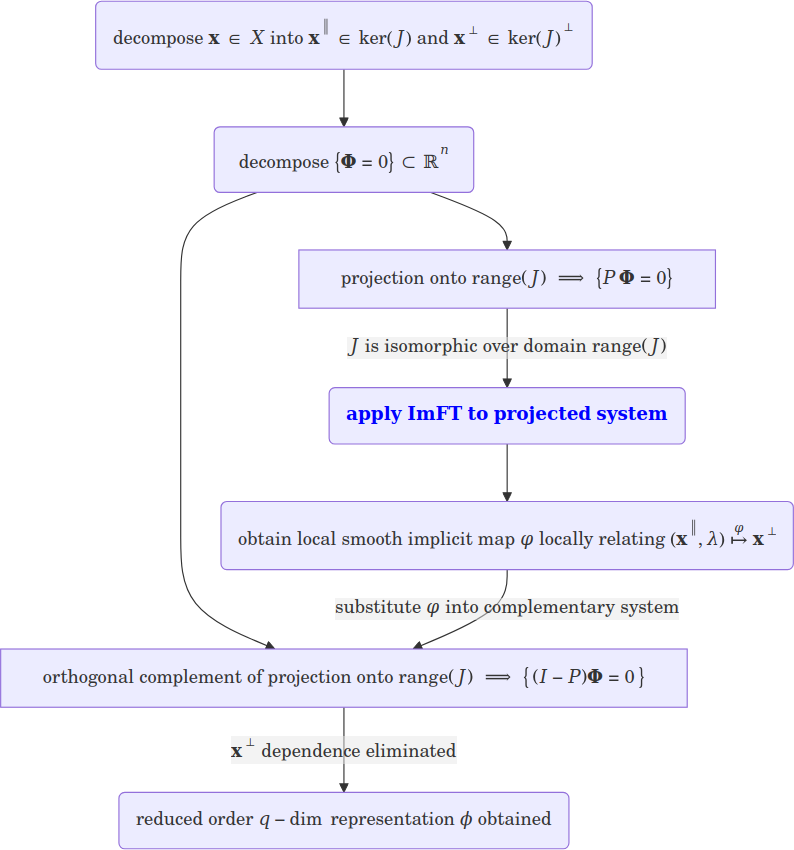
\includegraphics[width=\textwidth]{images/flowchart.png}
            \end{figure}
        \end{column}
    \end{columns}
\end{frame}

% \begin{frame}{Lyapunov Schmidt reduction}
%     \begin{block}{Procedure of Lyapunov Schmidt reduction}
%         \begin{enumerate}
%             \itemsep0em
%             \item Define the linear projection operator \(P:\mathbb{R}^n\to\mathrm{range}(J)\)
%             \item Draw the equivalence:
%                 \(
%                     \boldsymbol{\Phi}(\mathbf{x},\lambda) = 0\iff
%                     \begin{cases}
%                         P\boldsymbol{\Phi}(\mathbf{x},\lambda)      = 0 & \\
%                         (I-P)\boldsymbol{\Phi}(\mathbf{x},\lambda)  = 0 &
%                     \end{cases}
%                 \)
%             \item Restrict the domain of \(P\boldsymbol{\Phi}(\mathbf{x,\lambda})\) to \(\mathrm{range}(J)\) to force invertibility and apply the Implicit Function Theorem to it to find a smooth implicit local map satisfying \(\mathcal{N}(\mathbf{x}^\parallel_0,\lambda_0)\ni(\mathbf{x}^\parallel,\lambda)\mapsto\varphi(\mathbf{x}^\parallel,\lambda)=\mathbf{x}^\perp\in\mathcal{N}(\mathbf{x}^\perp_0)\)
%             \item Using \(\varphi\), eliminate the dependence on \(\mathbf{x}^{\perp}\) in \((I-P)\boldsymbol{\Phi}(\mathbf{x},\lambda) = 0\) to obtain a system of lower state dimension, whose solutions (zeros) are in one-to-one correspondence with the original system.
%         \end{enumerate}
%     \end{block}
%     In our work, we apply the bounds on the Implicit Function Theorem to the reduction step, which in turn establishes an estimate for the region of validity of the equivalence drawn between the original system and the recovered low-dimensional system.
% \end{frame}


% \begin{frame}{\section{Explicit Bounds on Lyapunov-Schmidt reduction}Explicit Bounds on Lyapunov-Schmidt reduction}
%     To state the bounds, we must compute the quantities \(M_x\), \(M_y\), \(\mathbf{L}_x(r_x)\), \(\mathbf{L}_{\mathbf{y}}(r_x,r_y)\) from (\ref{imftbounds}) in the framework of Lyapunov-Schmidt reduction
%     \begin{itemize}
%         % \item \(\ker(J)\times\ker(J)^{\perp}\times\mathbb{R}^m\ni(\mathbf{x}^\parallel,\mathbf{x}^\perp,\lambda)\mapsto\Xi(\mathbf{x}^\parallel,\mathbf{x}^\perp,\lambda):= \boldsymbol{\Phi}(\mathbf{x}^\parallel+\mathbf{x}^\perp,\lambda)\)
%         \item Consider orthonormal bases \(\{\mathbf{v}_1, \dots, \mathbf{v}_q\}\) of \(\ker(J)\), \(\{\mathbf{v}_1^{\perp}, \dots, \mathbf{v}_{n-q}^{\perp}\}\) of \(\ker(J)^{\perp}\) and \(\{\mathbf{w}_1, \dots, \mathbf{w}_{n-q}\}\) of \(\mathrm{range}(J)\), and define matrices %\(V\in\mathbb{R}^{n \times q}\), \(V^{\perp}\in\mathbb{R}^{n\times(n-q)}\) and \(W\in\mathbb{R}^{n\times(n-q)}\) as
%             \vspace{-3mm}\[
%                 {V = \begin{bmatrix} \mathbf{v}_1 & \dots & \mathbf{v}_q \end{bmatrix}}\quad{V^{\perp} = \begin{bmatrix} \mathbf{v}_1^{\perp} & \dots & \mathbf{v}_{n-q}^{\perp} \end{bmatrix}}\quad{W = \begin{bmatrix} \mathbf{w}_1, \dots, \mathbf{w}_{n-q}\end{bmatrix}}
%             \]\vspace{-4mm}
%         \item \(\boxed{M_{(\mathbf{x}^\parallel,\lambda)} := \norm{\begin{bmatrix}0 &W^{\top}D_\lambda\boldsymbol{\Phi}(\mathbf{x}_0,\lambda_0)\end{bmatrix}}}\) and \(\boxed{M_{\mathbf{x}^{\perp}} := \norm{(W^{\top} J V^{\perp})^{-1}}}\)
%         \item For \(r^\parallel,r^\perp>0\) let \({\mathcal{B}^\parallel:=\mathcal{B}\Big(\big(\mathbf{x}^\parallel_0,\lambda_0\big),r^\parallel\Big)}\) and \({\mathcal{B}^\perp:=\mathcal{B}\big(\mathbf{x}^\perp_0,r^\perp\big)}\)
%         \item Define \(\boxed{\mathbf{L}_{(\mathbf{x}^\parallel,\lambda)}(r^\parallel) := \sup\Big\{\norm{\xi_1}:(\mathbf{x}^\parallel,\lambda)\in\mathcal{B}^\parallel\Big\}}\) where
%         \vspace{-3mm}\[
%             {\xi_1 = W^{\top}\begin{bmatrix}D_{\mathbf{x}} \boldsymbol{\Phi}(\mathbf{x}^{\parallel}+\mathbf{x}^\perp_0,\lambda)V & D_{\lambda}\boldsymbol{\Phi}(\mathbf{x}^{\parallel}+\mathbf{x}^\perp_0,\lambda)-D_{\lambda}\boldsymbol{\Phi}(\mathbf{x}_0,\lambda_0)\end{bmatrix}}
%         \]\vspace{-4mm}
%         \item Let \({\xi_2(\mathbf{x}^{\parallel}, \mathbf{x}^{\perp},\lambda) = W^{\top}\big(D_{\mathbf{x}}\mathbf{\Phi}(\mathbf{x},\lambda)-J\big)V^{\perp}}\) and define
%             \vspace{-3mm}\[
%                 \boxed{\mathbf{L}_{\mathbf{x}^\perp}(r^\parallel,r^\perp) := \sup\Big\{\norm{\xi_2(\mathbf{x}^{\parallel}, \mathbf{x}^{\perp},\lambda)} : \Big((\mathbf{x}^\parallel,\lambda),\mathbf{x}^\perp\Big) \in\mathcal{B}^\parallel\times\mathcal{B}^\perp\Big\}}
%             \]\vspace{-4mm}
%     \end{itemize}
% \end{frame}


\begin{frame}{Explicit Bounds on Lyapunov-Schmidt reduction}
    \begin{columns}
        \begin{column}{0.25\textwidth}
            \begin{figure}[ht!]
                \centering
                \includesvg[width=0.75\textwidth]{images/varphi-LSR.svg}
                \caption{schematic of smooth implicit map \(\varphi:\mathcal{B}^\parallel\to\mathcal{B}^\perp\)}
            \end{figure}
        \end{column}
        \hfill
        \begin{column}{0.75\textwidth}
            Bounds of validity for reduced \(\dim\) map estimated at step where the Implicit Function Theorem is applied
            \begin{block}{Statement of Bounds}
                For any \(r^\parallel,r^\perp>0\) satisfying
                \vspace{-2mm}\[\begin{aligned}
                    \mathbf{L}_{(\mathbf{x}^\parallel,\lambda)}(r^\parallel)r^\parallel+\mathbf{L}_{\mathbf{x}^\perp}(r^\parallel,r^\perp)r^\perp & < \frac{r^\perp}{M_{\mathbf{x}^\perp}}-M_{(\mathbf{x}^\parallel,\lambda)}r^\parallel \\
                    M_{\mathbf{x}^\perp}\mathbf{L}_{\mathbf{x}^\perp}(r^\parallel,r^\perp) & < 1
                \end{aligned}\vspace{-2mm}\]
                \(\exists\) a smooth implicit map \(\varphi:\mathcal{B}^\parallel\to\mathcal{B}^\perp\) satisfying
                \vspace{-2mm}\[
                    \boldsymbol{\Phi}\big(\mathbf{x}^\parallel+\varphi(\mathbf{x}^\parallel,\lambda),\lambda\big) = 0 \quad\forall\,(\mathbf{x}^\parallel,\lambda)\in\mathcal{B}^\parallel
                \]
            \end{block}
            \(
                \boxed{M_x, M_y, r_x, r_y, \mathbf{L}_x, \mathbf{L}_{\mathbf{y}} \to M_{(\mathbf{x}^\parallel,\lambda)}, M_{\mathbf{x}^\perp}, r^\parallel, r^\perp, \mathbf{L}_{(\mathbf{x}^\parallel,\lambda)}, \mathbf{L}_{\mathbf{x}^\perp}}
            \)
            are respective \textcolor{blue}{translations of quantities} defined in slide [\ref{imftbounds}] \textcolor{blue}{into the Lyapunov-Schmidt reduction framework}.
        \end{column}
        \hfill
    \end{columns}
\end{frame}


% \begin{frame}{\section{Application}Application}
%     \begin{block}{}
%         \begin{itemize}
%             \item Analysis of bifurcations plays an important role in both \textit{understanding} and \textit{controlling} systems with complex non-linear features including power systems \cite{ajjarapu1992bifurcation}, epidemic processes \cite{pare2020modeling}, social dynamics \cite{bizyaeva2022nonlinear,bizyaeva2023thesis}, and neuromorphic computing networks \cite{juarez2024analysis}.
%             \item In a control context, objectives range from understanding when feedback laws give rise to bifurcations and potentially suppressing their onset \cite{chen1994overview,chen2000bifurcation}, to designing dynamics and feedback laws that give rise to meaningful behaviour through a bifurcation \cite{leonard2024fast}.
%         \end{itemize}
%     \end{block}
% \end{frame}


% \begin{frame}{Example: Recurrent Neural Network Model}
%     For \(\mathbf{x}=\begin{bmatrix}x_1&x_2\end{bmatrix}^{\top}\in\mathbb{R}^2\) and \(\lambda\in\mathbb{R}\), consider the dynamic model of the following two-node RNN described by
%     \(
%         \dot{\mathbf{x}} = -\mathbf{x}+\tanh\left(\begin{bmatrix}0&\lambda\\\lambda&0\end{bmatrix}\mathbf{x}\right)
%     \)
%     where \(\lambda\)'s magnitude regulates the slope of the saturation function \(\tanh\); the nodes are mutually excitatory if \(\lambda>0\) or mutually inhibitory if \(\lambda<0\).
%     \begin{figure}[ht!]
%         \centering
%         \begin{subfigure}{.4\textwidth}
%             \centering
%             \includesvg[width=\textwidth]{images/0_9.svg}
%         \end{subfigure}%
%         \begin{subfigure}{.4\textwidth}
%             \centering
%             \includesvg[width=\textwidth]{images/1_1.svg}
%         \end{subfigure}
%         \caption{system flow around the pitchfork bifurcation at origin near \(\lambda_0=1\)}
%     \end{figure}
% \end{frame}


% \begin{frame}{\section{Example: Recurrent Neural Network Model}Example: Recurrent Neural Network Model}
%     \begin{block}{Results}
%         \(\forall\;\boxed{r^{\perp}>0, r^{\parallel}\in(0,2)}\:\exists\) smooth implicit map
%         \(\varphi:\mathcal{B}\big((0,1),r^\parallel\big)\to\mathcal{B}(0,r^\perp)\) 
%         \vspace{-4mm}\[\text{satisfying }
%             \boxed{\varphi(\alpha\mathbf{v}_{1},\lambda)+\frac12\begin{bmatrix}1&-1\\-1&1\end{bmatrix}\tanh\Big(\lambda\big(\alpha\mathbf{v}_1-\varphi(\alpha \mathbf{v}_{1},\lambda)\big)\Big) = 0}
%         \vspace{-4mm}\]
%         yielding
%         \(\boxed{g(\alpha,\lambda) = -\alpha+\mathbf{v}_1^{\top}\tanh\Big[\lambda\big(\alpha\mathbf{v}_1-\varphi(\alpha\mathbf{v}_{1},\lambda)\big)\Big]},\mathbf{v_1}=\begin{bmatrix}\frac{1}{\sqrt2}&\frac{1}{\sqrt2}\end{bmatrix}^{\top}\)
%     \end{block}
% \end{frame}

\begin{frame}{\section{Example: Recurrent Neural Network model}Example: Recurrent Neural Network model}
    \begin{columns}[T] % align columns
        \begin{column}{.24\textwidth}
            \begin{figure}[ht!]
                \centering
                \includesvg[width=\textwidth]{images/0_9.svg}
                \includesvg[width=\textwidth]{images/1_1.svg}
                \caption{system flow around pitchfork bifurcation at origin near \(\lambda_0=1\)}
            \end{figure}
        \end{column}%
        \hfill%
        \begin{column}{.78\textwidth}
            \textbf{System}: for \(\mathbf{x}=\begin{bmatrix}x_1&x_2\end{bmatrix}^{\top}\in\mathbb{R}^2\) and \(\lambda\in\mathbb{R}\), consider the dynamic model of the following two-node RNN:
            \vspace{-2mm}\[
                \dot{\mathbf{x}} = -\mathbf{x}+\tanh\left(\begin{bmatrix}0&\lambda\\\lambda&0\end{bmatrix}\mathbf{x}\right)
            \vspace{-2mm}\]
            % where \(\lambda\)'s magnitude regulates the slope of the saturation function \(\tanh\); the nodes are mutually excitatory if \(\lambda>0\) or mutually inhibitory if \(\lambda<0\).
            \textbf{Final values of bound parameters}:
            \begin{itemize}
                \item \(\boxed{M_{(\mathbf{x}^\parallel,\lambda)} = 0}\), \(\boxed{\mathbf{L}_{(\mathbf{x}^\parallel,\lambda)}(r^\parallel)=0}\), \(\boxed{M_{\mathbf{x}^\perp} = \frac{1}{2}}\)
                \item \(\boxed{\begin{aligned}
                    \mathbf{L}_{\mathbf{x}^\perp}(r^\parallel,r^\perp) &= \tiny\{1-\min(0,\lambda):\\&\left(\frac{1}{\sqrt{2}}(x_1+x_2),\lambda\right)\in\mathcal{B}\big((0,1),r^\parallel\big)\}\\&=1-(1-r^\parallel)=r^\parallel
                \end{aligned}}\)
            \end{itemize}
        \end{column}%
        \hfill
    \end{columns}
\end{frame}

\begin{frame}{Example: Recurrent Neural Network model}
    \begin{center}
        \alert{Substituting the parameters} finally yields \(\boxed{r^\perp\in\mathbb{R}^+}\) and \(\boxed{r^\parallel\in(0,2)}\)
    \end{center}
    \begin{block}{Results}
        Let \(\mathbf{v}=\frac{1}{\sqrt2}\begin{bmatrix}1&1\end{bmatrix}^{\top}\). For \textcolor{blue}{\(\boxed{\mathbf{r^{\perp}>0, r^{\parallel}\in(0,2)}}\)} we have the implicit map \textcolor{blue}{\(\varphi:\mathcal{B}\big((0,1),r^\parallel\big)\to\mathcal{B}(0,r^\perp)\)} satisfying
        \vspace{-2mm}\[
            \boxed{\varphi(\alpha\mathbf{v},\lambda)+\frac12\begin{bmatrix}1&-1\\-1&1\end{bmatrix}\tanh\Big(\lambda\big(\alpha\mathbf{v}-\varphi(\alpha \mathbf{v},\lambda)\big)\Big) = 0}
        \vspace{-2mm}\]
        yielding reduced \(\dim\) system
        \(\boxed{g(\alpha,\lambda) = -\alpha+\mathbf{v}^{\top}\tanh\Big[\lambda\big(\alpha\mathbf{v}-\varphi(\alpha\mathbf{v},\lambda)\big)\Big]}\)
    \end{block}
\end{frame}

\begin{frame}{Example: RNN model (maximal bounding ball)}
    \begin{figure}[ht!]
        \centering
        \includesvg[width=0.8\textwidth]{images/RNN.svg}
        \caption{bifurcation diagram for illustrated 2-node RNN model}
    \end{figure}
\end{frame}

\begin{frame}{Extensions and Future Plans}
    \begin{itemize}
        \item Application to higher dimensional systems including nonlinear opinion dynamics \cite{bizyaeva2022nonlinear}\footfullcite{bizyaeva2022nonlinear} to explore how the graph structure affects the tightness of the established bounds.
        \item Extension to infinite-dimensional systems, since the Lyapunov Schmidt reduction is defined more generally for Fredholm operators over Banach spaces.
    \end{itemize}
\end{frame}

\end{document}